\documentclass[10pt,a4paper]{book}
\usepackage{a4} % 297x210 paper
\usepackage{amsmath}
\usepackage{amssymb} % Some extra symbols
\usepackage{makeidx} % If you want to generate an index, automatically
\usepackage{graphicx} % If you want to include postscript graphics
\usepackage{color}
\usepackage{multicol}
\usepackage{pifont}
\usepackage{url}
\usepackage{titlesec}
\usepackage{titletoc}
\usepackage{cite}
\usepackage{scalefnt}
\usepackage{fancyhdr}
\usepackage{wrapfig}
\usepackage{charter}
\usepackage[british]{babel}
\usepackage{lscape}
\usepackage{hyperref}
\usepackage{listings}
\hypersetup{
  colorlinks,%
  citecolor=blue,%
  filecolor=black,%
  linkcolor=black,%
  urlcolor=black,%
  pdftex=true,%
  breaklinks=true}
\usepackage{listings}
\lstset{language=bash,basicstyle=\small,breaklines=false}
\usepackage{subfigure}
\usepackage[font=small,labelfont=bf,textfont=it]{caption}
\titlespacing*{\section}{0pt}{1.5cm plus 0.2cm minus 0.2cm}{0.5cm}
\titlespacing*{\subsection}{0pt}{1.2cm plus 0.2cm minus 0.2cm}{0.5cm}
\titlespacing*{\subsubsection}{0pt}{1.0cm plus 0.2cm minus 0.2cm}{0.5cm}
\titleformat*{\section}{\usefont{T1}{pag}{db}{n}\selectfont\large}
\titleformat*{\subsection}{\usefont{T1}{pag}{db}{n}\selectfont\large}
\titleformat*{\subsubsection}{\sf\selectfont\large}

\definecolor{Grey}{rgb}{0.40,0.60,0.80}

\titleformat{\chapter}[display]
{\normalfont\huge\sf}
{\flushright\vspace{1cm}{\Huge\color{Grey}\thechapter\vspace{0.2cm}\hrule}}
{10pt}
{\vspace{-2.2cm}\scalefont{1.15}}

\setlength{\footskip}{1.5cm}
% Define footer for chapter start pages
\fancypagestyle{plain}{
  \fancyhf{}
  \cfoot{}
  \fancyfoot[r]{\sf\bfseries\thepage}
}

\pagestyle{fancy}

\renewcommand{\headrulewidth}{0pt}

% Change TOC style
\titlecontents{chapter}[0pt]
  {\addvspace{1.5pc}}
  {\contentsmargin{0pt} \sf \makebox[0pt][r]
  {\color{Grey}\Huge\thecontentslabel\enspace} \large}
  {\contentsmargin{0pt} \large}
  {\bfseries\hfill\contentspage}
  [\color{Grey}\hrule\addvspace{0.6pc}]

\contentsmargin{2.0em}

\titlecontents{section}[5em]   {\contentslabel{2.3em}}{}{}{\hfill\contentspage}
\titlecontents{subsection}[9em]{\contentslabel{3em}}{}{}{\hfill\contentspage}

\newenvironment{fancyfig}
{
	\begin{figure}[float]
	\begin{center}
}
{
	{\color{Grey}\vspace{0.2cm}\hrule}
	\end{center}
	\end{figure}
}

\topmargin=-0.3in
\textheight=8.93in
\oddsidemargin=0.57in
\evensidemargin=0.57in
\textwidth=5.71in
\renewcommand{\headwidth}{\textwidth}

\makeatletter
\renewcommand{\@seccntformat}[1]{\llap{\csname the#1\endcsname\hskip1em}}

\renewcommand{\maketitle}{\pagestyle{empty}%
  \begin{titlepage}%
       \vspace{5cm}
        \hspace{-4.5cm}%
        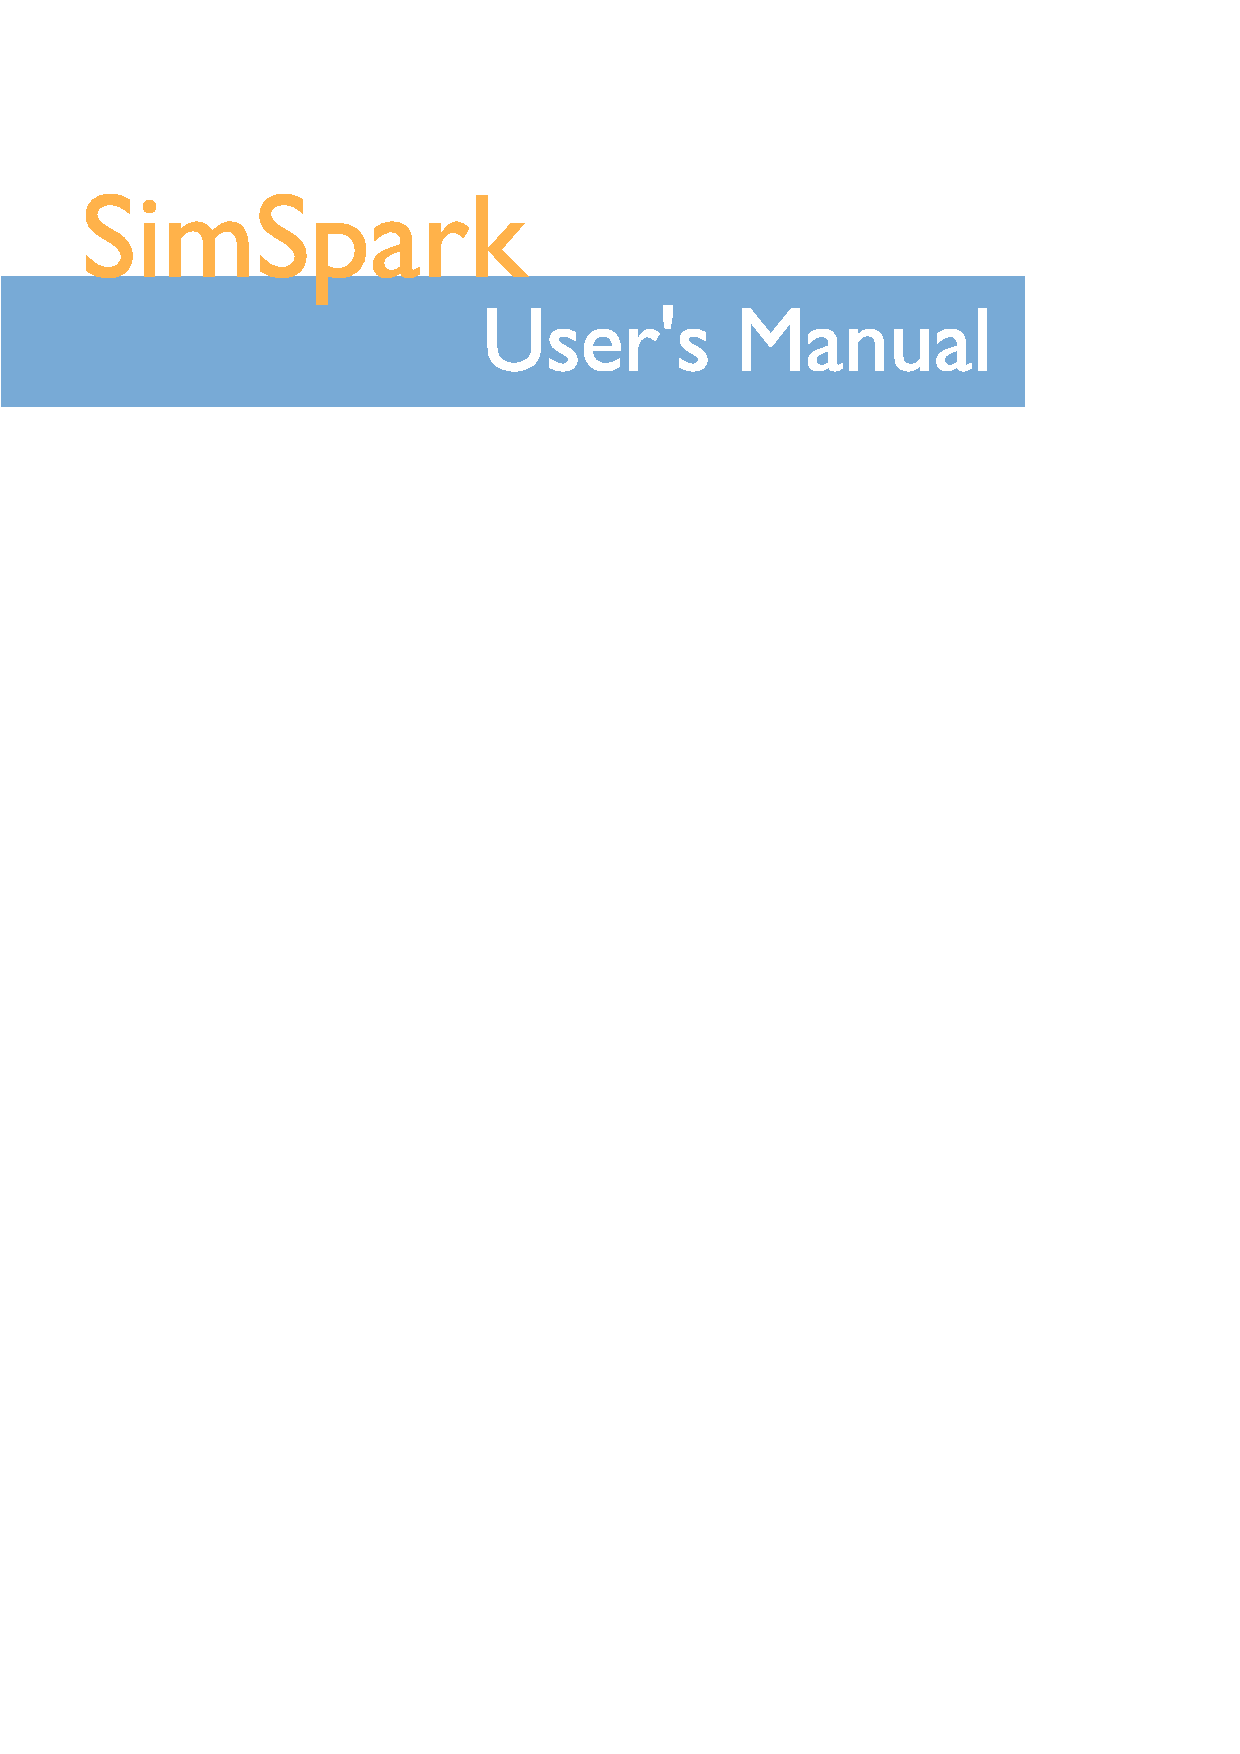
\includegraphics{fig/header}\hfill%
         \vspace*{0.1cm}
         \hspace*{-2.5cm}%  
         \begin{minipage}[t]{0.5\linewidth}
         		\textsf{\Large
         			\flushleft{%
				\textit{Edited by:}\\%
				Joschka Boedecker\\%
				Klaus Dorer\\%
				Markus Rollmann\\%
				Yuan Xu\\%
				Feng Xue\\%
				Marian Buchta\\%
				Hedayat Vatankhah\\%
				Stefan Glaser\\%
			}
		}
	\end{minipage}
	\hspace*{6cm}
	\begin{minipage}[t]{0.5\linewidth}
	\textsf{\Large\flushright{Version 1.3}}
         \end{minipage}
	
	\vspace{-4.5cm}
		
	\begin{minipage}[t]{\linewidth}
	\hspace*{2.25cm}
	
\includegraphics[width=16cm]{fig/simsparklogo}
	\end{minipage}
	
	\vspace*{-0.25cm}
	\hspace*{-3cm}%
	\begin{minipage}[b]{3cm}
	\textsf{\Large\flushleft{August 2010}}
        	\end{minipage}
	
  \end{titlepage}%
}

\makeatother
\pagestyle{fancy}
\lhead{}
\rhead{}
\cfoot{}
\rfoot{\sf\bfseries\thepage}


% Define new language for Server message listings.
\definecolor{darkgreen}{rgb}{0, 0.6, 0}
\lstdefinelanguage{SSML} {
   basicstyle=\ttfamily,
   sensitive=true,
   breaklines=true,
   stringstyle=\color{flexred},
   alsoletter={0, 1, 2, 3, 4, 5, 6, 7, 8, 9, -},
   keywords=[1]
   {
     teamRed, teamBlue, BeforeKickOff, 1000-501
   }, keywordstyle={[1]\color{red}},
   keywords=[2]
   {
     time, now, GS, t, pm, hear, self, GYR, rt, ACC, a, HJ, UJ, See, G1R, G2R,
     G1L, G2L, F1R, F2R, F1L, F2L, FRP, TCH, val, pol, team, id, n, ax, c, f,
     B, P, ax1, ax2
   }, keywordstyle={[2]\color{blue}},
   keywords=[3] 
   {
     head, llowerarm, rlowerarm, lfoot, rfoot, lf, rf, torso, hj1, hj2, laj1,
     raj1, laj2, raj2, laj3, raj3, laj4, raj4, llj1, rlj1, llj2, rlj2, llj3,
     rlj3, llj4, rlj4, llj5, rlj5, llj6, rlj6, laj1_2, raj1_2, llj2_3, rlj2_3,
     llj5_6, rlj5_6
   }, keywordstyle={[3]\color{darkgreen}}, 
}

